\section{Target group analysis}\label{sec:target-group-analysis}

Chess as a game has a broad appeal, as it is played by many people, young and old.
As previously stated, chess has risen in popularity recently, so it is sufficed to say that the user group is a lot
larger than it was a few years ago.
Therefore, it is necessary to analyze the target group to narrow down the scope of the project.

A good way to do just that is by splitting the target group into different categories.
It is possible to split the people that play chess by age, skill level, and how frequently they play.
As the project is about the learning process of chess, dividing the target group by skill level is the most relevant.
In that case, our target group is beginners.

% textidote: ignore begin

\begin{figure}
    \centering
    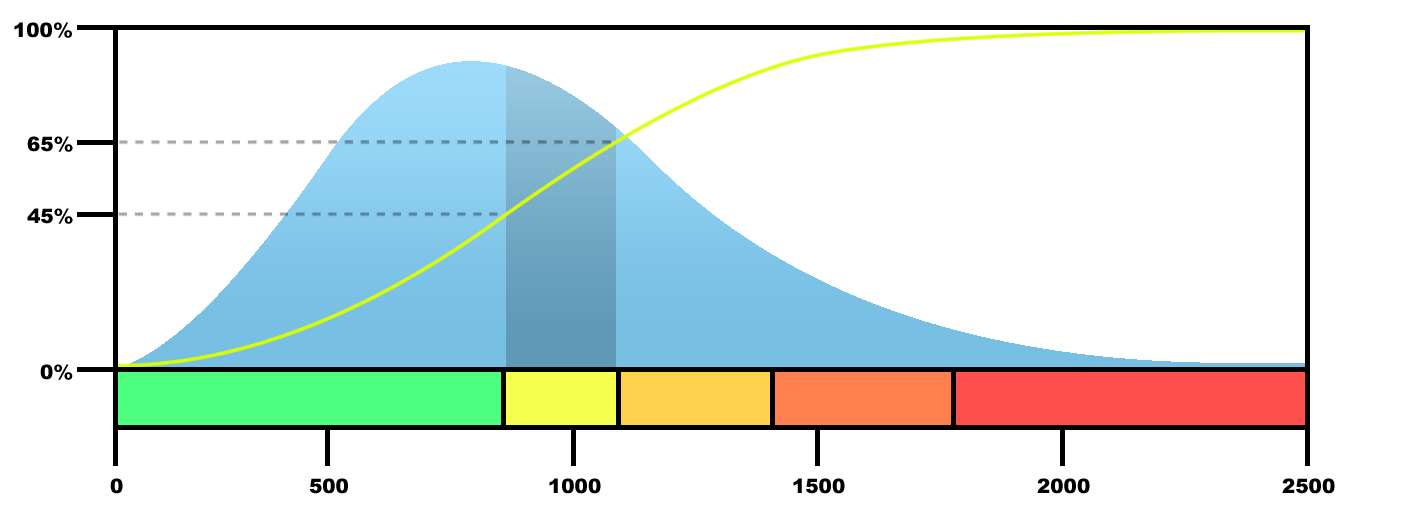
\includegraphics[width=1\textwidth]{chess-graph}
    \caption{Rating distribution graph based off of Chess.com's rating system~\cite{chess-ratings}.}\label{fig:graph}
\end{figure}

The Figure~\ref{fig:graph} shows a graph made to illustrate different skill levels amongst Chess.com's user base.
The blue wave represents the amount of users with a certain rating.
We don't have direct numbers, as Chess.com's graph that this is based on is very limited in terms of data.
The color bars on the bottom represent different skill groups, which are taken from ChessGoals~\cite{chess-ratings}.

% textidote: ignore end

The first group, which is marked in green, the biggest one, is novices. 
They are not expected to know much about chess or its rules, so they are not fit to be our target group, because our 
goal is not to teach the rules of chess, but to help people improve their skills.
The second group, which is marked in yellow, is beginners.
This is our main target group, as they are the ones that are expected to benefit the most from our product.
The graph peaks at the end of the novices group, which means that transitioning from novice to beginner seems to be the 
hardest challenge for new players.
The third and fourth groups, which are marked in light and dark orange, are intermediate 1 and 2 players.
While they are not our main target group, they may still have a subset of the problems that the beginners have.
The last group, which is marked in red, is expert players.
Unlike intermediate players, they are less likely to benefit from our product.

The yellow line shows the percentage of the user base that a specific rating can beat.
For example, an expert player can beat close to 100\% of the user base, while someone who is just starting out can't
beat anyone.
Taking a look at our target group, it can be seen that it starts at 45\% and ends at 65\%.
Our goal will therefore be to ease the transition from 45\% to 65\% and beyond.
